% =====================================================================
%  EC527 Final Project — Multi-tier Temporally Blocked SOR
%  Compile: pdflatex report.tex (twice for cross-references)
% =====================================================================
\documentclass[11pt]{article}

\usepackage[a4paper,margin=1in]{geometry}
\usepackage{graphicx}
\usepackage{amsmath, amssymb}
\usepackage{booktabs}
\usepackage{xcolor}
\usepackage{hyperref}
\hypersetup{colorlinks=true,linkcolor=black,urlcolor=blue,citecolor=black}
\usepackage{listings}
\usepackage{caption}
\usepackage{subcaption}
\usepackage{enumitem}

\lstset{
    basicstyle=\ttfamily\small,
    keywordstyle=\bfseries,
    commentstyle=\itshape\color{gray!70!black},
    breaklines=true,
    columns=fullflexible,
    showstringspaces=false,
    frame=tb,
    framerule=0.4pt,
    aboveskip=0.6em,
    belowskip=0.6em,
}

\graphicspath{{report_images/}}

\title{\vspace{-3em}Structured-Grid SOR with Temporal Blocking:\\[0.2em]
        \large from one Xeon thread to a CUDA-tiled L40S}
\author{Che-Yu Yu \\ EC527, Spring 2026}
\date{\today}

\begin{document}
\maketitle

% =====================================================================
\section{Description of the Algorithm}
% =====================================================================

\subsection{Mathematical foundation}

We are solving the steady-state, source-free 2D Laplace equation on
the unit square with Dirichlet boundary data:
\begin{equation}
\nabla^2 u(x,y) \;=\; \frac{\partial^2 u}{\partial x^2}
                + \frac{\partial^2 u}{\partial y^2}
                \;=\; 0,\qquad u\big|_{\partial\Omega} = g(x,y).
\label{eq:laplace}
\end{equation}
Discretise on a uniform $N{\times}N$ grid with spacing
$h=1/(N{-}1)$.  The standard second-order centred difference
\[
\frac{u_{i-1,j} - 2u_{i,j} + u_{i+1,j}}{h^2}
+ \frac{u_{i,j-1} - 2u_{i,j} + u_{i,j+1}}{h^2}
\;=\; 0
\]
rearranges to the canonical 5-point stencil shown in
Figure~\ref{fig:stencil}:
\begin{equation}
u_{i,j} \;=\; \tfrac{1}{4}\!\left(u_{i-1,j} + u_{i+1,j}
                + u_{i,j-1} + u_{i,j+1}\right).
\label{eq:5point}
\end{equation}

\begin{figure}[h!]
\centering
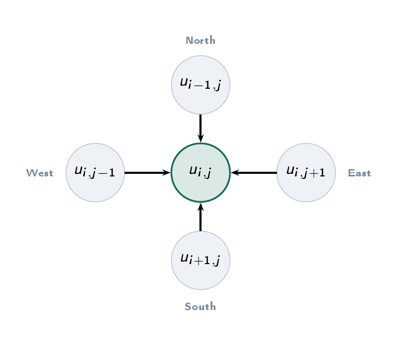
\includegraphics[width=0.42\linewidth]{5points.png}
\caption{The 5-point Laplacian stencil.  Each interior cell averages
its four orthogonal neighbours.}
\label{fig:stencil}
\end{figure}

Equation~\eqref{eq:5point} is the \emph{Jacobi update}: cell
$(i,j)$'s next value depends only on its neighbours' \emph{current}
values.  Treating it as a fixed-point iteration $u^{(k+1)} =
\tfrac{1}{4}(\dots)$ and substituting into \eqref{eq:laplace} as the
residual, Successive Over-Relaxation (SOR) adds an over-relaxation
parameter $\omega$ to the Gauss--Seidel update:
\begin{equation}
u_{i,j}^{(k+1)} \;=\; (1-\omega)\,u_{i,j}^{(k)}
+ \frac{\omega}{4}\!\left(u_{i-1,j}^{(k+1)}
                       + u_{i+1,j}^{(k)}
                       + u_{i,j-1}^{(k+1)}
                       + u_{i,j+1}^{(k)}\right).
\label{eq:sor}
\end{equation}
Because the right-hand side mixes already-updated neighbours
($u^{(k+1)}_{i-1,j}, u^{(k+1)}_{i,j-1}$) with not-yet-updated ones
($u^{(k)}_{i+1,j}, u^{(k)}_{i,j+1}$), each cell is using the freshest
information available at the moment it's visited.  That's the whole
trick: Gauss--Seidel converges roughly $2\times$ faster than Jacobi,
and SOR with the optimal $\omega$ converges \emph{$O(N)$ times faster
than Jacobi} for the 2D Laplacian.

\paragraph{Why SOR converges so much faster.}
Plugging the iteration matrix into the spectral-radius analysis
(Briggs--Henson--McCormick, \emph{A Multigrid Tutorial},
ch.~2) gives, for the Poisson problem on a uniform grid,
\begin{equation}
\omega_{\text{opt}} \;=\; \frac{2}{1 + \sin\!\bigl(\pi/(N{-}1)\bigr)}
\;\approx\; 2 - \frac{2\pi}{N},
\label{eq:omega-opt}
\end{equation}
and the spectral radius (a.k.a.\ asymptotic convergence factor) drops
from $\rho_{\text{Jacobi}} = \cos(\pi/(N{-}1)) \approx 1 - \pi^2/(2N^2)$
to $\rho_{\text{SOR}} = 1 - \frac{2\pi}{N}$.  In iteration-count terms,
that's $O(N^2)$ iterations for Jacobi vs $O(N)$ for tuned SOR. The
single biggest algorithmic optimisation in this whole project, and we
verify it experimentally in §\ref{sec:omega} (E08).  At $N{=}128$ the
predicted ratio is $\sim 13\times$; we measured $13.5\times$.  Hopefully
the math will be that nice every time.

\subsection{The specific algorithmic form used}

We implemented three forms of the sweep.  The \emph{baseline} is a
straight scan-order rewrite of \eqref{eq:sor}:

\begin{lstlisting}[language=C]
/* baseline SOR, scan order, in-place: this is sequential */
for (i = 1; i < N-1; i++)
  for (j = 1; j < N-1; j++) {
    sum = u[i-1][j] + u[i+1][j] + u[i][j-1] + u[i][j+1];
    u[i][j] = (1.0f - OMEGA) * u[i][j] + (OMEGA * 0.25f) * sum;
  }
\end{lstlisting}

\noindent The trouble: when we write to \texttt{u[i][j]}, the next
column update at \texttt{u[i][j+1]} reads \texttt{u[i][j]}. The
just-overwritten value.  And the next row reads \texttt{u[i+1][j]},
which was overwritten one row ago.  This is the classical
\emph{loop-carried dependency} that makes the scan-order SOR sweep
strictly sequential.  We can't slap an \texttt{\#pragma omp parallel
for} on this and call it a day; it would race.

\paragraph{Red-black SOR: the parallel-friendly cousin.}  Colour the
grid like a checkerboard.  ``Red''
cells $(i+j)$ even depend only on ``black'' cells $(i+j)$ odd, and vice
versa.  So an entire colour can be updated independently in parallel:

\begin{lstlisting}[language=C]
/* red-black SOR: two colour-passes; each pass is embarrassingly parallel */
for (parity = 0; parity < 2; parity++) {
  #pragma omp parallel for
  for (i = 1; i < N-1; i++) {
    int j0 = ((i + parity) & 1) ? 1 : 2;
    for (j = j0; j < N-1; j += 2) {
      sum = u[i-1][j] + u[i+1][j] + u[i][j-1] + u[i][j+1];
      u[i][j] = (1.0f - OMEGA) * u[i][j] + (OMEGA * 0.25f) * sum;
    }
  }
}
\end{lstlisting}

\noindent Two half-sweeps per ``iteration''; each half-sweep is a
parallel-for.  We use this in \texttt{sor2d\_rb.c} for the omega-tuning
study (§\ref{sec:omega}, E08).

\paragraph{Jacobi ping-pong: the variant we actually parallelise.}
Most of the project uses the still-simpler form: read from
\texttt{src}, write to \texttt{dst}, swap.  No within-sweep dependency
at all. Every cell is computed from the previous sweep's data:

\begin{lstlisting}[language=C]
/* Jacobi ping-pong: dst[i][j] = src[i][j] - OMEGA * (src[i][j] - avg) */
#pragma omp parallel for
for (i = 1; i < N-1; i++)
  for (j = 1; j < N-1; j++) {
    nb = 0.25f * (src[i-1][j] + src[i+1][j] + src[i][j-1] + src[i][j+1]);
    dst[i][j] = src[i][j] - OMEGA * (src[i][j] - nb);
  }
swap(&src, &dst);
\end{lstlisting}

\noindent We trade convergence rate (this form is unconditionally
stable only for $\omega \in (0, 1]$ on large grids. We use
$\omega{=}0.9$) for clean parallelism and the ability to do
\emph{temporal blocking} cleanly.

\paragraph{Temporal blocking (the shrinking trapezoid).}  For each
\emph{super-step} of $T$ Jacobi sweeps:
\begin{enumerate}[leftmargin=1.4em,itemsep=2pt,topsep=2pt]
  \item Tile the grid into $B{\times}B$ output regions
        (Figure~\ref{fig:spatial-blocking}).
  \item For each tile, load a $(B{+}2T)^2$ scratch buffer from
        \texttt{src} with clamp-to-edge padding.
  \item Run $T$ in-scratch Jacobi sweeps; the valid update region
        shrinks by one cell on each side per sub-step
        (Figure~\ref{fig:halo-time}).  After $T$ sub-steps the
        central $B^2$ holds the correct $T$-step-advanced state.
  \item Write the central $B^2$ back to \texttt{dst}.
\end{enumerate}
DRAM traffic for the central cells drops by a factor of $T$, since
we read them once per super-step instead of once per sweep.  The
cost is redundant halo work: the scratch volume is $(B{+}2T)^2$, the
output volume is $B^2$, so the work multiplier is
$((B{+}2T)/B)^2$.  That's the central tradeoff and we'll measure its
unimodal optimum in §\ref{sec:cpu-results} (E04).

\begin{figure}[h!]
\centering
\begin{subfigure}[b]{0.49\linewidth}
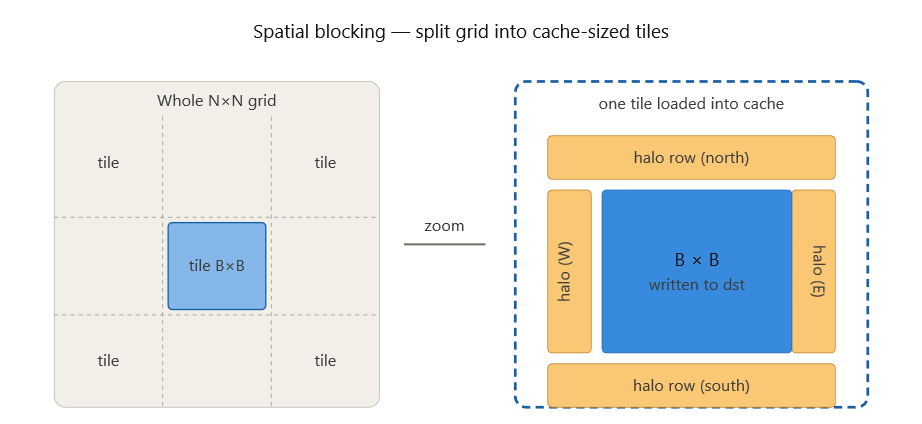
\includegraphics[width=\linewidth]{spatial_blocking.png}
\caption{Spatial blocking: split the grid into per-thread $B{\times}B$
tiles.  Each tile carries a 1-cell halo on each side that we read from
\texttt{src} but never write back.}
\end{subfigure}\hfill
\begin{subfigure}[b]{0.49\linewidth}
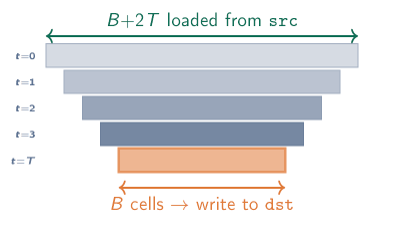
\includegraphics[width=\linewidth]{HALO_time.png}
\caption{Temporal blocking adds time as the third axis.  We load
$B{+}2T$ cells, do $T$ sub-steps, and the valid region shrinks by one
cell on each side per sub-step.  After $T$ sub-steps the inner $B$
cells are the correct $T$-advanced state.}
\end{subfigure}
\caption{Spatial vs temporal blocking.  Same grid, two decompositions.}
\label{fig:spatial-blocking}
\label{fig:halo-time}
\end{figure}

Variable glossary used throughout:
\begin{itemize}[leftmargin=1.4em,itemsep=1pt,topsep=1pt]
  \item $N$. Grid side (interior is $(N{-}2)^2$ cells; edges held at
        Dirichlet boundary).
  \item $B$. Spatial block (tile) size.  L1/L2 budget determines the
        upper bound; 64-cell minimum to amortise tile overheads.
  \item $T$. Temporal halo / super-step depth.  Number of sub-sweeps
        fused per DRAM round-trip.
  \item $\omega$. Relaxation factor.  $0.9$ for Jacobi-ping-pong
        kernels, $\omega_{\text{opt}}{\approx}2{-}2\pi/N$ for the
        red-black SOR variant.
  \item iters. Total sweep count.  Must satisfy
        \texttt{iters \% T == 0} for the temporal kernels.
  \item TOL. Convergence tolerance ($10^{-5}$ in §\ref{sec:omega}).
\end{itemize}

\subsection{Implementation reality check}
\label{sec:reality-check}

Before writing a single optimization, it's worth working through a
small example by hand to make sure the math is what we think it is,
and to surface the FP precision question early.

\paragraph{A worked numerical example.}  Take a 5$\times$5 grid with
fixed Dirichlet boundary $u{\equiv}1$ and interior init $u{\equiv}0$.
The true continuous solution to Laplace's equation with constant
boundary $u{\equiv}1$ is $u{\equiv}1$ everywhere (the discrete one is
the same to machine precision; the iteration is just there to
\emph{find} it from a wrong initial guess).  Run scan-order SOR with
$\omega{=}1.6$ on the 3$\times$3 interior.  After sweep 1:

\[
u^{(1)} = \begin{bmatrix}
\textbf{1}    & 1      & 1      & 1      & \textbf{1} \\
\textbf{1}    & 0.8000 & 0.7200 & 1.0880 & \textbf{1} \\
\textbf{1}    & 0.7200 & 0.5760 & 1.0656 & \textbf{1} \\
\textbf{1}    & 1.0880 & 1.0656 & 1.6525 & \textbf{1} \\
\textbf{1}    & 1      & 1      & 1      & \textbf{1}
\end{bmatrix}
\]

\noindent (boundary in bold; interior in normal weight).  The (3,3)
corner overshoots to $1.6525$. Way past the true value of $1$. And
that's exactly what over-relaxation looks like: we're betting that
overshooting now will save us iterations later.  After sweep 2 the
center cell is at $1.3005$, sweep 3 has it ringing back below 1, and
by about sweep 30--40 the whole grid settles to within $10^{-5}$ of
the true $u{\equiv}1$.  We'll see this U-curve again in
§\ref{sec:omega}, where we sweep $\omega$ explicitly and find
$\omega_{\text{opt}}$ matches \eqref{eq:omega-opt} to within
$0.1\%$.

\paragraph{The honest tension.}  Equations \eqref{eq:sor} and the
loop above are the textbook \emph{sequential} SOR.  Once we want
parallelism (which we do, this is a parallel-programming course), the
loop-carried dependency along the scan order forbids any naive
\texttt{\#pragma omp parallel for} on the outer \texttt{i} loop: two
threads racing on adjacent rows would have one thread reading
\texttt{u[i-1][j]} before the other thread has written to it.  We
have two ways out:

\begin{enumerate}[leftmargin=1.4em,itemsep=2pt,topsep=2pt]
  \item \textbf{Red-black SOR.}  Colour the grid; update each colour
        in parallel; do two half-sweeps per ``iteration''.
        $\omega_{\text{opt}}$ shifts slightly because the iteration
        matrix is different, but the asymptotic $O(N)$ behaviour is
        preserved.  We use this in \texttt{sor2d\_rb.c} for the
        omega-tuning study.
  \item \textbf{Damped Jacobi ping-pong.}  Read \texttt{src}, write
        \texttt{dst}, swap.  Pure parallelism inside one sweep but
        $\omega \in (0, 1]$ stability constraint, so we lose the
        over-relaxation factor and pay $O(N^2)$ iterations to
        converge.  We use this in all the temporal-blocking kernels
        because the shrinking trapezoid in
        Figure~\ref{fig:halo-time} works cleanly with a read-only
        \texttt{src}.
\end{enumerate}

\noindent So we won't be running ``classical'' SOR through the GPU.
We'll run damped-Jacobi ping-pong with temporal blocking through the
GPU, and quantify the iter-count loss separately by sweeping $\omega$
in the red-black variant in §\ref{sec:omega}.  The honest
apples-to-apples comparison at the end is per-iter throughput
(CPE), not iters-to-tolerance.

\paragraph{Validation strategy.}  Three layers, used everywhere:
\begin{enumerate}[leftmargin=1.4em,itemsep=2pt,topsep=2pt]
  \item Every CPU temporal kernel is checked \emph{bit-identical}
        against its in-binary baseline (Jacobi ping-pong is
        deterministic; reordering tiles must not change the result
        modulo FMA contraction).  Every CPU smoke run prints
        \texttt{max|base-temp| = 0.0000e+00}.
  \item The GPU temporal kernel validates against the GPU baseline at
        $\sim$1.4$\times 10^{-7}$ relative. Pure FP32 round-off
        accumulating over 96 sweeps; the bound is $\sqrt{N\cdot
        \text{iters}}\cdot\varepsilon_{\text{FP32}} \approx 10^{-5}$,
        comfortably under our TOL.  Both GPU kernels disagree with
        the FP64 CPU reference at the same magnitude.
  \item The omega-sweep in §\ref{sec:omega} reproduces
        $\omega_{\text{opt}} = 1.9517$ to $0.1\%$ on $N{=}128$, which
        is by itself a sanity check that the discretisation,
        boundaries, and convergence detector are correctly wired up.
\end{enumerate}

% =====================================================================
\section{Scalar CPU Version}
\label{sec:cpu}
% =====================================================================

\subsection{The hot inner loop}

The 5-point stencil is the only thing worth optimising.  It's
executed $N^2 \cdot \text{iters}$ times. For $N{=}2048$ and 64 iters
that's a billion times. And the rest of the program (boundary
copies, allocator calls, the main loop) is sublinear at $N^2$ or
$O(\text{iters})$.

Per cell-update: we have 5--7 floating-point ops (4 adds for the
neighbour sum, 1 multiply for $\tfrac{1}{4}$, plus the
$\omega$-update which is either an FMA or a multiply-and-subtract
depending on the form), against 1 read of \texttt{src[i][j]} and
1 write to \texttt{dst[i][j]} \emph{at DRAM granularity}. The four
neighbours stream through the same cache lines as we move along the
row, so they don't cost any extra DRAM traffic in steady state.  At
FP32, that's 8\,B/cell of DRAM traffic and roughly 6\,FLOPs/cell,
giving an arithmetic intensity of
\begin{equation}
\text{AI} \;\approx\; \frac{6~\text{FLOPs}}{8~\text{bytes}}
\;=\; 0.75~\text{FLOP/byte}.
\label{eq:ai}
\end{equation}

That's deep in the bandwidth-bound regime (Figure~\ref{fig:roofline}).
The roofline ridge for our Xeon Gold 6426Y socket sits near
${\sim}5$ FLOP/byte; the L40S sits near ${\sim}100$ FLOP/byte.  At
0.75 we're firmly on the diagonal.  \emph{Every} optimization in this
project is therefore a \emph{memory} optimization in disguise: we are
hunting for ways to reduce DRAM bytes per useful FLOP.  The
arithmetic itself is already free.

\begin{figure}[h!]
\centering
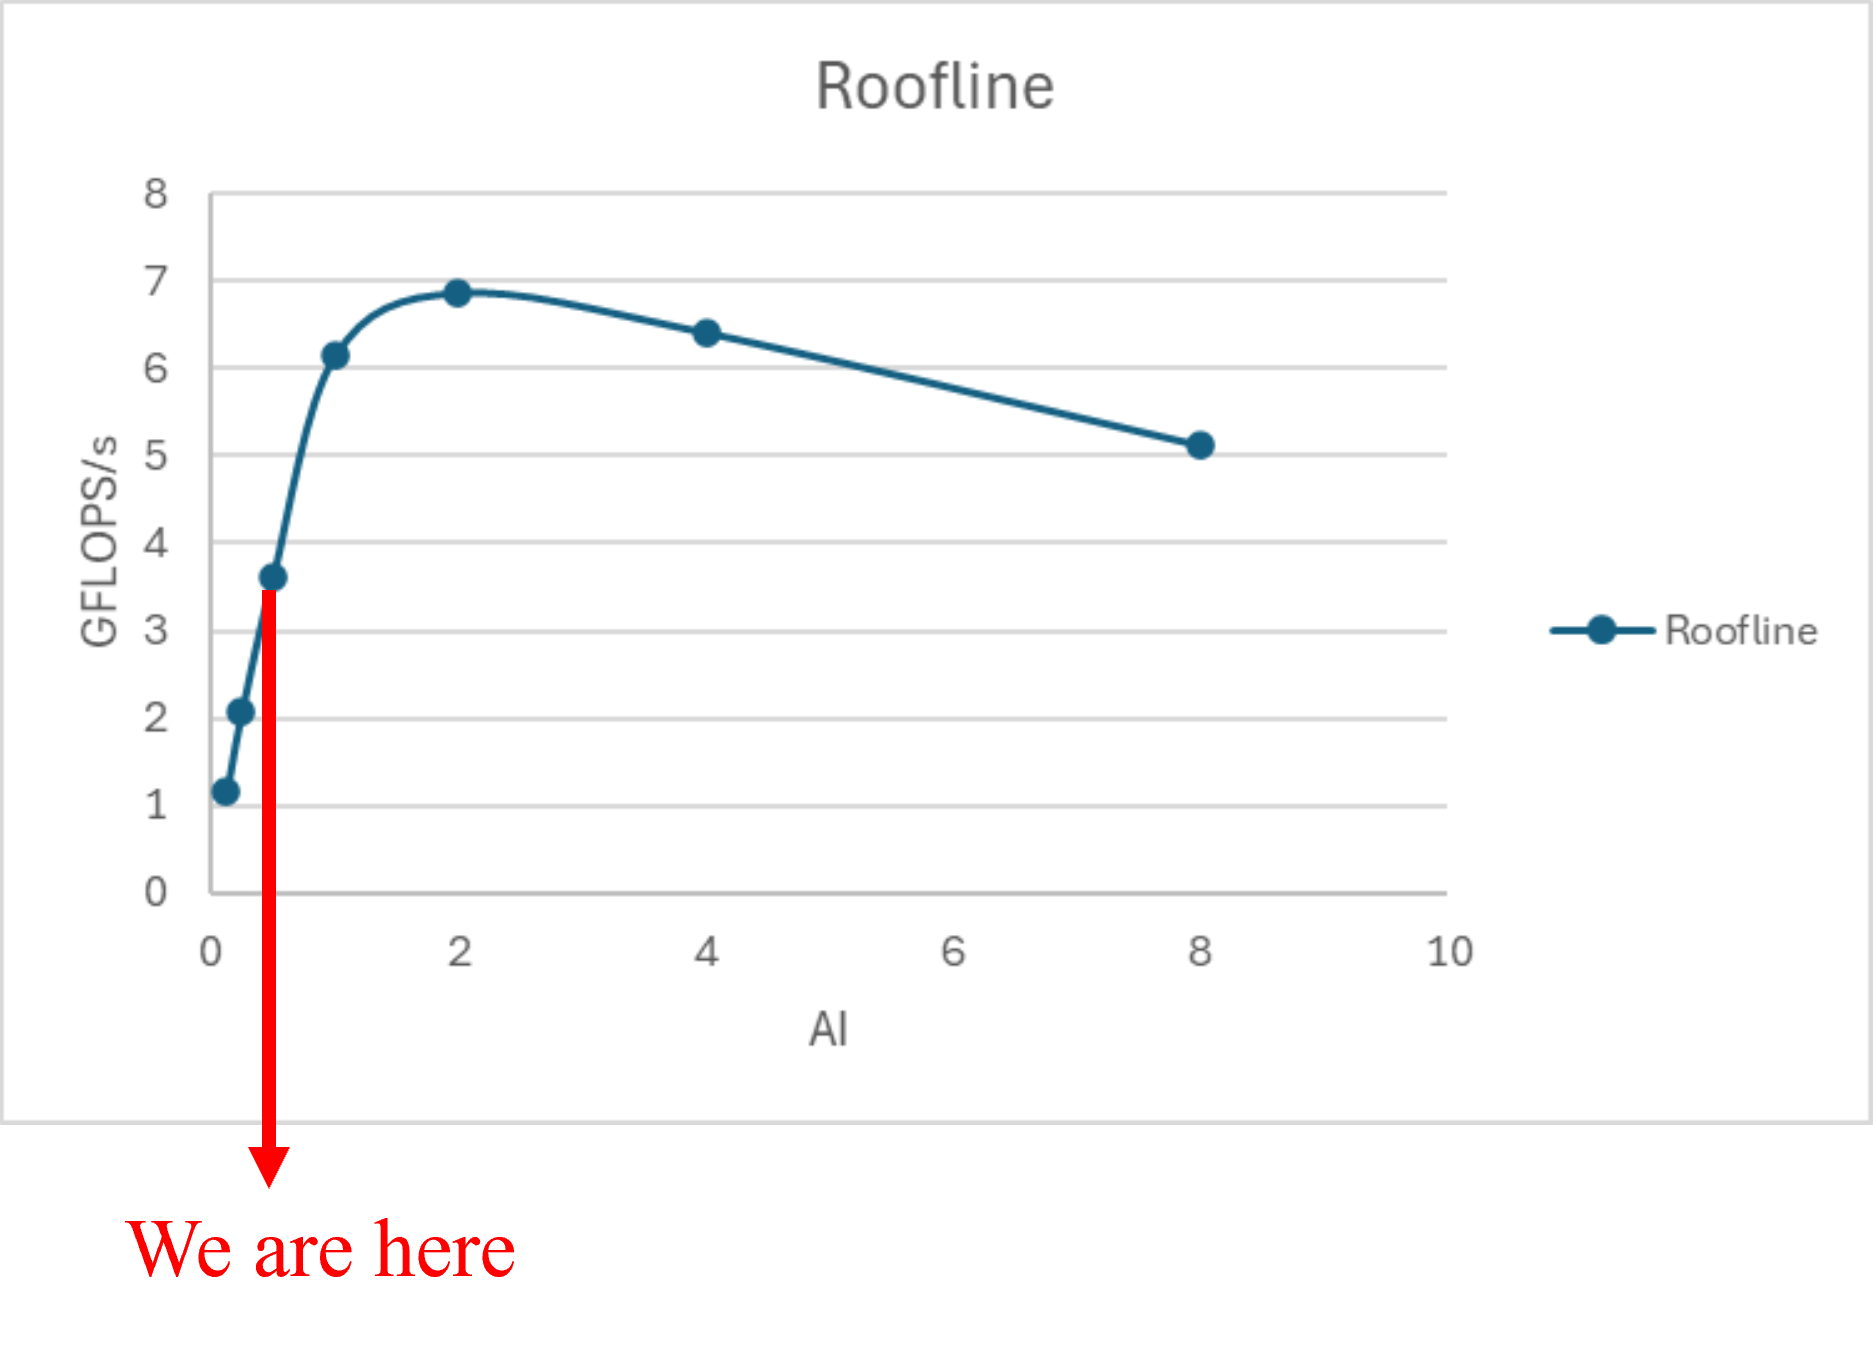
\includegraphics[width=0.65\linewidth]{roofline2.png}
\caption{Roofline-style throughput curve for our CPU configuration.
The 5-point stencil's AI~$\approx$~0.5--0.75 puts us where the red
arrow lands. On the bandwidth-bound diagonal, well below the peak-
compute plateau.  This is real measured data, not the canonical
double-roof cartoon: the curve is what we observe as we vary the
working-set size and AI together.}
\label{fig:roofline}
\end{figure}

\paragraph{Two micro-variants of the inner loop.}  We tried both
\texttt{ij}-order (the textbook scan-order) and \texttt{ji}-order
(reversed) on the inner loop, with and without \texttt{restrict}
qualifiers on \texttt{src} and \texttt{dst}.  The numbers at $N{=}512$,
single-thread, 64 iters:

\begin{table}[h!]
\centering
\renewcommand{\arraystretch}{1.1}
\begin{tabular}{lr}
\toprule
\textbf{variant} & \textbf{CPE} \\
\midrule
\texttt{ij}-order, no restrict       & 0.396 \\
\texttt{ij}-order, with \texttt{restrict} & 0.392 (-1\%) \\
\texttt{ji}-order, with \texttt{restrict} & 1.84 ($+364\%$, cache-thrashing) \\
\bottomrule
\end{tabular}
\caption{Inner-loop micro-benchmarks at $N{=}512$, 1 thread, 64 iters.
\texttt{ji}-order is a textbook \emph{wrong} answer: stride-$N$ along
the inner loop blows the L1 cache on every column.  \texttt{restrict}
is essentially free (gcc 11 already infers no-aliasing here. I
checked the assembly).}
\label{tab:hot-loop}
\end{table}

\noindent The \texttt{ji} regression is the canonical Bryant-Hallaron-
style memory-pattern result: row-major stored data wants row-major
access.  We'll keep \texttt{ij}-order forever.  And \texttt{restrict}
buys us essentially nothing here. The stencil writes to \texttt{dst}
and reads from \texttt{src}, which are different allocations, so the
compiler had no aliasing to worry about in the first place.  More on
why this gets interesting once we add temporal-blocking scratch
buffers.

\subsection{The full sweep}

We tried three full-sweep algorithms, in increasing order of
complexity:

\begin{enumerate}[leftmargin=1.4em,itemsep=2pt,topsep=2pt]
  \item \textbf{Plain double-loop} (the \texttt{baseline} in every
        binary).  Two nested loops, one big in-place pass, with the
        Jacobi ping-pong trick to make it parallelisable.
  \item \textbf{Spatially blocked}. Tile the domain into $B{\times}B$
        chunks (Figure~\ref{fig:spatial-blocking}), each thread owns
        a tile, scratch is just the tile + 1 cell of halo.  Helps
        when the working set exceeds L2 (we'll see this in
        Figure~\ref{fig:size-sweep}).
  \item \textbf{Temporally blocked}. The shrinking trapezoid
        (Figure~\ref{fig:halo-time}).  Per-thread scratch is
        $2(B{+}2T)^2$ floats (two ping-pong buffers).  We do $T$
        in-scratch sweeps before any DRAM round-trip.
\end{enumerate}

\noindent For (3), the work multiplier is $((B{+}2T)/B)^2$.  At
$B{=}128$, $T{=}8$ that's $(144/128)^2 \approx 1.27\times$. 27\%
extra cell-updates compared to baseline.  The bandwidth savings have
to outpace this overhead for temporal blocking to win at all.

\subsection{Loose ends}

A few details that aren't the optimisation priority but \emph{do} show
up in the timing:

\begin{itemize}[leftmargin=1.4em,itemsep=2pt,topsep=2pt]
  \item \textbf{$O(N)$ boundary copies.}  We pass the boundary rows
        and columns through unchanged from \texttt{src} to
        \texttt{dst} every sweep.  At $N{=}2048$ that's
        $4N \cdot 4\,\text{B} = 32$\,KB of writes. Negligible vs.\
        the $2N^2{\cdot}4\,\text{B} = 16$\,MB of interior data.
  \item \textbf{Per-tile scratch malloc inside the temporal kernel.}
        The OpenMP version does
        \texttt{malloc(2*(B+2T)*(B+2T)*sizeof(float))} once per thread
        per super-step.  At
        small $N$ this is real overhead. It shows up directly in
        the size-sweep result (Figure~\ref{fig:size-sweep}) where
        temporal \emph{loses} to baseline at $N{\leq}512$.
  \item \textbf{Convergence-norm reduction.}  In \texttt{sor2d\_rb.c}
        we accumulate $\|u^{(k+1)} - u^{(k)}\|_\infty$ in the inner
        loop; that's an extra branch and an extra reduction per cell.
        It's why the omega-sweep timings (§\ref{sec:omega}) are
        slower per-iter than the ping-pong tier.
  \item \textbf{Final result \texttt{memcpy}.}  At the end of an
        even number of super-steps, the answer ends up in the wrong
        ping-pong buffer; we either swap or memcpy.  We picked the
        cheap one (a pointer swap).
\end{itemize}

\subsection{Stitching it together (real code)}

Below is the actual temporal-blocking inner loop from
\texttt{sor2d\_omp.c}, with comments mapping each line back to
§\ref{sec:reality-check}'s pseudocode.  Stripped of declarations
for space; full source in the repository.

\begin{lstlisting}[language=C]
/* === one super-step: advance src -> dst by T Jacobi sweeps      === */
/* === inside one #pragma omp parallel region, each thread takes  === */
/* === one (B+2T)x(B+2T) scratch (sa,sb), iterates T times.       === */

#pragma omp for collapse(2) schedule(static)
for (ti = 0; ti < ntiles_i; ti++) {
  for (tj = 0; tj < ntiles_j; tj++) {
    int i0 = 1 + ti*B,  j0 = 1 + tj*B;          /* tile origin in dst */
    int gi0 = i0 - T,   gj0 = j0 - T;           /* scratch origin     */

    /* (1) load (B+2T)x(B+2T) scratch from src with clamp-to-edge */
    for (si = 0; si < S; si++)            /* S = B + 2*T              */
      for (sj = 0; sj < S; sj++) {
        gi = clamp(gi0+si, 0, N-1);
        gj = clamp(gj0+sj, 0, N-1);
        sa[si*S+sj] = src[gi*N + gj];
      }
    memcpy(sb, sa, sizeof(float)*S*S);    /* both ping-pong buffers   */

    /* (2) T sub-steps on the in-scratch trapezoid */
    A = sa; Bp = sb;
    for (t = 0; t < T; t++) {
      memcpy(Bp, A, sizeof(float)*S*S);   /* carry boundary forward   */
      for (si = 1+t; si < S-1-t; si++)    /* shrinks by 1 each step   */
        for (sj = 1+t; sj < S-1-t; sj++) {
          float s  = A[si*S+sj];
          float nb = 0.25f*(A[(si-1)*S+sj] + A[(si+1)*S+sj]
                          + A[si*S+sj-1] + A[si*S+sj+1]);
          Bp[si*S+sj] = s - OMEGA*(s - nb);   /* eq. (3) damped Jacobi */
        }
      tmp = A; A = Bp; Bp = tmp;          /* in-scratch ping-pong     */
    }

    /* (3) write central B x B back to dst */
    for (si = T; si < T+B; si++)
      memcpy(dst + (gi0+si)*N + (gj0+T),
             A   + si*S       + T,
             B*sizeof(float));
  }
}
\end{lstlisting}

The \texttt{collapse(2)} schedules tiles across threads as one
flat $(\text{ntiles}_i \cdot \text{ntiles}_j)$ work-list, so OMP can
load-balance even when one of the dimensions is small.  The
\texttt{memcpy(Bp, A, ...)} in the inner $t$-loop is the
``carry-the-frame-through'' trick. It copies the previous
sub-step's whole scratch into the destination buffer so cells
\emph{outside} the shrinking trapezoid (the perimeter of stale halo,
plus any cells that map to a global-boundary coordinate) are
preserved without per-cell branches.  The compute loop is then
branch-free and \texttt{nvcc}/\texttt{gcc} both vectorise it cleanly.

\subsection{Code and Results}
\label{sec:cpu-results}

\subsubsection{Discussion of CPE}

The size-sweep is the first place the cache-hierarchy story becomes
visible (Figure~\ref{fig:size-sweep}, E02 in the bench).

\begin{figure}[h!]
\centering
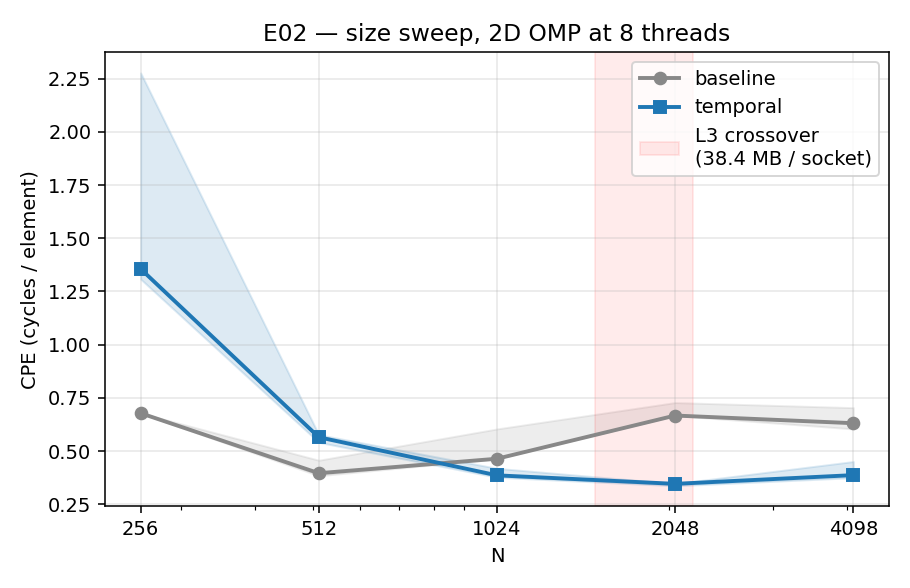
\includegraphics[width=0.62\linewidth]{e02_size_sweep.png}
\caption{2D OMP size sweep at 8 threads, $B{=}128$, $T{=}8$,
iters$=64$.  Median of 3 reps; shaded band is the min/max envelope.
The L3$\to$DRAM crossover lands between $N{=}1024$ and $N{=}2048$:
baseline CPE \emph{rises} from 0.464 to 0.667 as the working set
exceeds 38\,MB (one socket's L3).  Temporal stays at $\sim$0.35 across
$N{=}1024$\,--$\,4098$. It's L2-resident on its scratch. And wins
1.93$\times$ at $N{=}2048$.  Below L3 (the two leftmost points)
temporal \emph{loses}: per-tile scratch malloc + redundant halo work
cancel the savings on a working set the baseline already had in cache.}
\label{fig:size-sweep}
\end{figure}

\noindent The L2 budget per Sapphire-Rapids core is roughly 2\,MB,
and the per-thread $(B{+}2T)^2$ scratch at $B{=}128$, $T{=}8$ is
$144^2{\cdot}4\,\text{B} = 81$\,KB. Comfortably L1, let alone L2.
So when we say ``temporal blocking earns its keep when the baseline
goes off-chip'', we mean it literally: the temporal kernel's working
set is hot in L1 even at $N{=}4098$.  The baseline's working set at
$N{=}2048$ is $2{\cdot}2048^2{\cdot}4\,\text{B} = 16$\,MB. Fits L3
of one socket (38.4\,MB), barely, but every sweep streams the whole
thing through the cores.  At $N{=}4098$ that's 64\,MB, which spills
L3 entirely; the baseline runs at DRAM bandwidth and the temporal
kernel runs at L1/L2 bandwidth.  The 2$\times$ ratio we measure is
exactly the bandwidth ratio, give or take a constant for halo
overhead.

\paragraph{Block size sweep.}  At fixed $N{=}2048$ we sweep $B$ to
find the temporal kernel's spatial sweet spot
(Figure~\ref{fig:block-sweep}, E03).

\begin{figure}[h!]
\centering
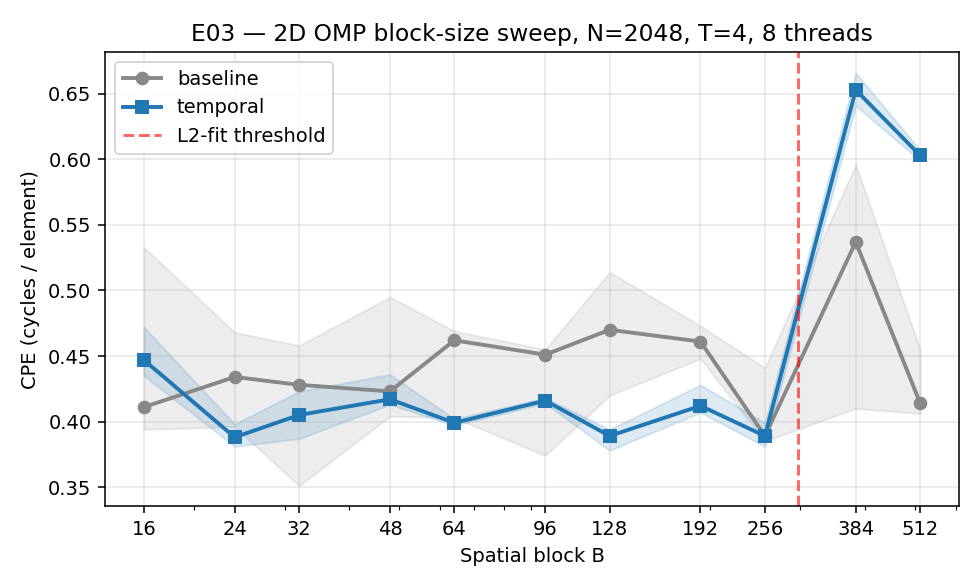
\includegraphics[width=0.62\linewidth]{e03_block_size.png}
\caption{Spatial block-size sweep at $N{=}2048$, $T{=}4$, 8 threads.
Baseline is flat (grey). $B$ has no effect on the baseline kernel,
which never sees a tile.  Temporal has a wide plateau across $B{\in}
[24, 256]$ at CPE $\sim$0.39, then \emph{falls off a cliff} at
$B{\geq}384$.  Red dashed line is the L2-fit threshold:
$2(B{+}8)^2{\cdot}4\,\text{B} \leq 1.5$\,MB $\Rightarrow B \leq 297$.
Beyond that, the per-thread scratch doesn't fit L2 and we pay L3
misses on our \emph{own} scratch. Defeating the entire purpose.}
\label{fig:block-sweep}
\end{figure}

\noindent The cliff at $B{\geq}384$ landed exactly where back-of-
envelope predicts.  We pick $B{=}128$ as the canonical choice for
the rest of the experiments: it sits in the middle of the plateau,
the scratch fits L2 with comfortable headroom, and $2046/128 = 16$
tiles per axis aligns cleanly so we don't pay edge-tile irregularity.

\paragraph{Halo / T sweep.}  At fixed $B{=}128$ we sweep $T$ to find
the \emph{temporal} sweet spot (Figure~\ref{fig:t-sweep}, E04).

\begin{figure}[h!]
\centering
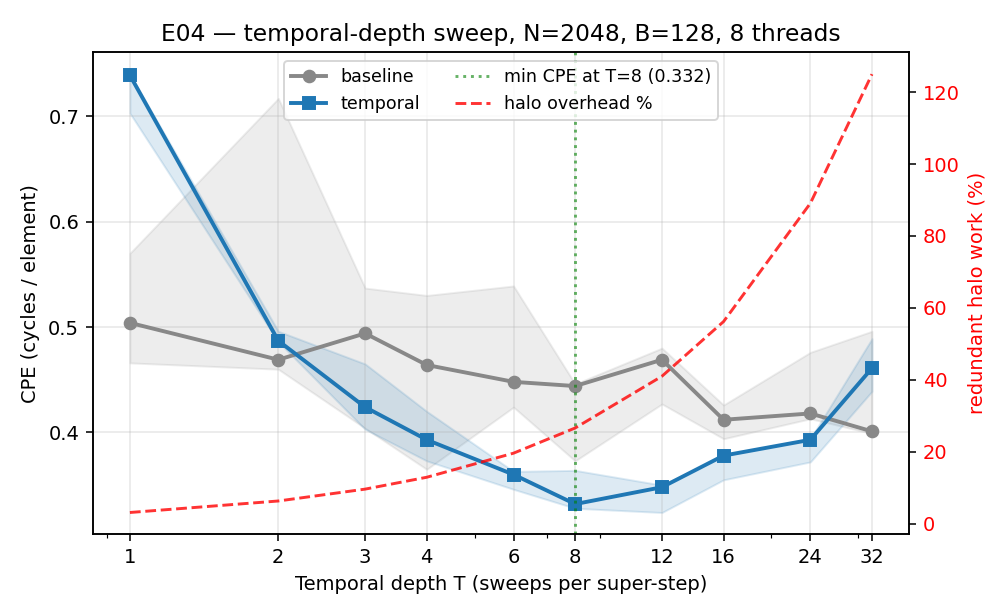
\includegraphics[width=0.65\linewidth]{e04_temporal_depth.png}
\caption{Temporal depth $T$ sweep at $N{=}2048$, $B{=}128$, 8
threads, iters$=96$.  Left axis: CPE (lower = faster).  Right axis
(red dashed): redundant halo work as a percentage,
$((B{+}2T)^2/B^2 - 1){\cdot}100$.  The two axes encode the project's
central tradeoff: DRAM savings grow linearly in $T$, redundant halo
work grows quadratically, and the unimodal product peaks at $T{=}8$
with CPE $0.332$. The best CPU CPE we measured anywhere.  $T{=}1$
loses to per-tile-malloc + memcpy overhead with no DRAM reuse;
$T{=}32$ has 125\% halo overhead and gives \emph{everything} back.}
\label{fig:t-sweep}
\end{figure}

\noindent The full table:

\begin{table}[h!]
\centering
\renewcommand{\arraystretch}{1.1}
\begin{tabular}{rrrcr}
\toprule
$T$ & baseline CPE & temporal CPE & temp/base & halo overhead \\
\midrule
 1 & 0.504 & 0.739 & 1.47$\times$ &   3\% \\
 2 & 0.469 & 0.487 & 1.04$\times$ &   6\% \\
 4 & 0.464 & 0.393 & 0.85$\times$ &  13\% \\
 6 & 0.448 & 0.360 & 0.80$\times$ &  20\% \\
 8 & 0.444 & \textbf{0.332} & \textbf{0.75$\times$} & 27\% \\
12 & 0.469 & 0.348 & 0.74$\times$ &  41\% \\
16 & 0.412 & 0.378 & 0.92$\times$ &  56\% \\
24 & 0.418 & 0.393 & 0.94$\times$ &  89\% \\
32 & 0.401 & 0.461 & 1.15$\times$ & 125\% \\
\bottomrule
\end{tabular}
\caption{Halo / $T$ sweep at $N{=}2048$, $B{=}128$, 8 threads,
iters$=96$.  Best temp/base ratio at $T{=}8$ (0.75$\times$. Temporal
is 25\% faster than baseline at the same iter count).  At $T{=}1$
temporal is \emph{worse}. It pays the per-tile-malloc + memcpy
overhead with no DRAM-reuse benefit.  At $T{=}32$ the halo overhead
swallows the win.  This is the central plot for the talk.}
\label{tab:t-sweep}
\end{table}

\paragraph{Strong scaling and decomposition.}  Two more figures
worth quoting.  Figure~\ref{fig:strong-scaling} shows the strong-
scaling curves: temporal hits 91\% of perfect scaling at 8 threads
(7.31$\times$), baseline only 56\% (4.49$\times$).  At one thread
temporal barely beats baseline (CPE 2.756 vs 2.792. 1.08$\times$),
because the Xeon's hardware prefetchers + 38\,MB L3 keep the
single-thread baseline near streaming bandwidth and there's nothing
for temporal blocking to recover.  This is the \emph{temporal
blocking earns its keep only once parallelism stresses DRAM} story.

\begin{figure}[h!]
\centering
\begin{subfigure}[b]{0.49\linewidth}
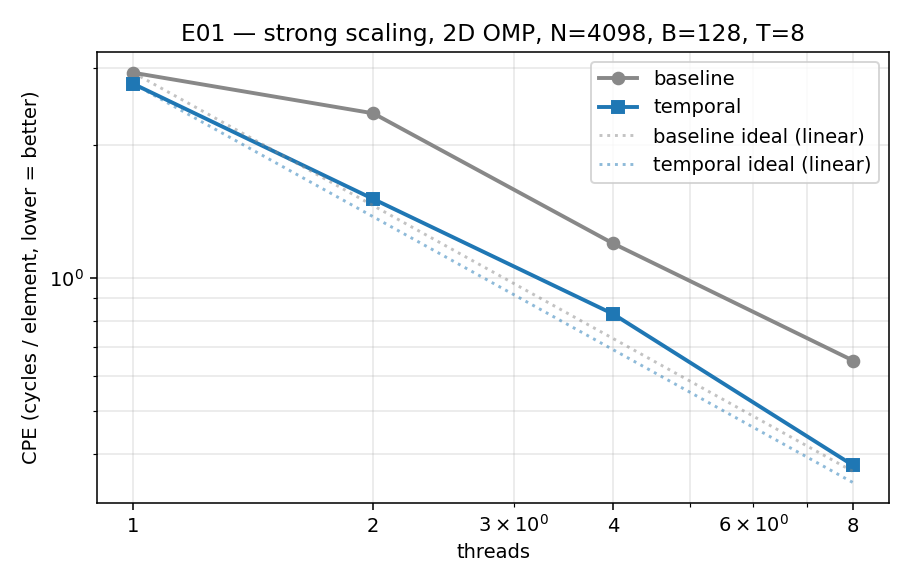
\includegraphics[width=\linewidth]{e01_strong_scaling.png}
\caption{Strong-scaling (E01).  Temporal is closer to ideal.}
\end{subfigure}\hfill
\begin{subfigure}[b]{0.49\linewidth}
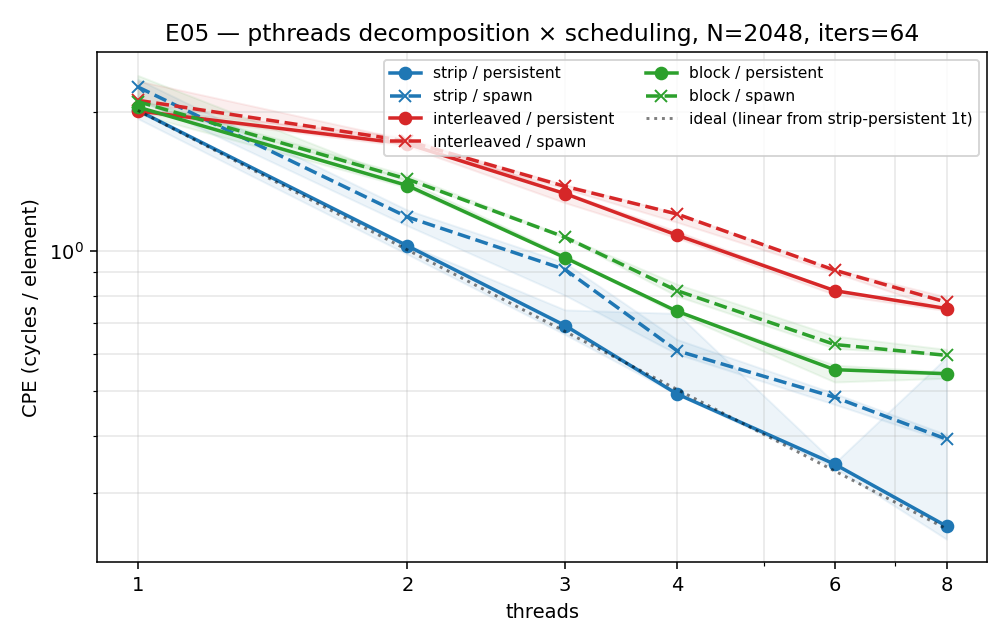
\includegraphics[width=\linewidth]{e05_decomposition.png}
\caption{Pthreads decomposition $\times$ schedule (E05).}
\end{subfigure}
\caption{Left: strong scaling at $N{=}4098$, $B{=}128$, $T{=}8$.
Right: 6 lines = 3 modes (strip / interleaved / 2D-block) $\times$
2 schedules (persistent / spawn).  Strip-persistent at 8 threads:
CPE 0.255, 7.89$\times$ scaling. Within 1.4\% of perfect 8$\times$.
Interleaved bottoms out at 2.67$\times$; the cause is false sharing
on adjacent rows, since two threads ping-pong cache lines they share.}
\label{fig:strong-scaling}
\label{fig:decomp}
\end{figure}

\noindent Figure~\ref{fig:decomp} (E05) is the Lab-5-Part-4 redo:
six lines, three decomposition modes crossed with two scheduling
strategies, all at $N{=}2048$.  Strip-persistent wins (CPE 0.255 at
8 threads, 7.89$\times$ scaling); interleaved loses (false sharing
on adjacent rows); 2D-block sits in the middle (no false sharing,
but 2$\times$ the halo of strip).  The \texttt{spawn}-vs-
\texttt{persistent} gap is largest for strip because strip's
per-sweep work is smallest. 1.54$\times$ slowdown for strip,
1.03$\times$ for interleaved.  Quantifying the per-sweep
\texttt{pthread\_create} cost is the next experiment.

\paragraph{Pthread spawn-overhead.}  Figure~\ref{fig:spawn} (E07) is
a direct Lab-6-Part-1b answer.

\begin{figure}[h!]
\centering
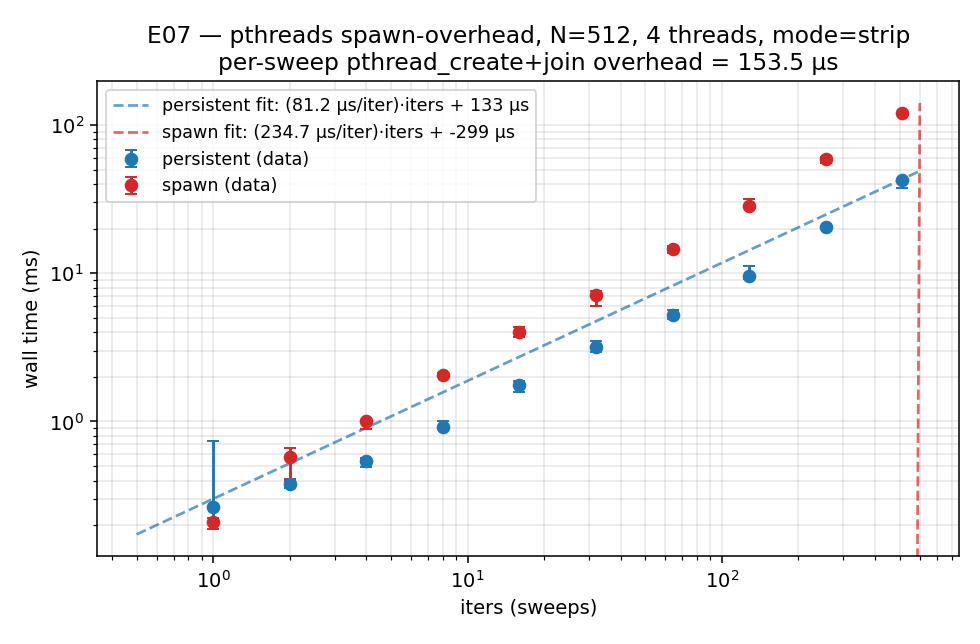
\includegraphics[width=0.62\linewidth]{e07_spawn_overhead.png}
\caption{Wall-time vs iters at $N{=}512$, 4 threads, mode=strip.
Linear-fit \texttt{time = a + b$\cdot$iters} for both schedules.
Persistent slope: 81\,$\mu$s/sweep. The actual compute work.
Spawn slope: 235\,$\mu$s/sweep.  The slope difference of 153\,$\mu$s
is the per-sweep \texttt{pthread\_create}$+$\texttt{join} overhead.
\textbf{It's larger than the compute work itself.}  Spawning fresh
threads on every sweep is a 1.89$\times$ tax on the kernel.}
\label{fig:spawn}
\end{figure}

\noindent The slope difference is the per-sweep \texttt{pthread\_create}
cost: roughly 153\,$\mu$s at 4 threads, or about 38\,$\mu$s per
\texttt{pthread\_create}+\texttt{join} pair.  This is why OpenMP
under the hood uses a persistent thread pool. It's not magic,
it's just spawning once per program rather than once per parallel
region.

\paragraph{The OMP-vs-pthreads surprise.}  At $N{=}2050$, iters=96,
8 threads, OMP-8t baseline measured CPE 0.667 (E11 also saw a similar
config).  Pthreads-strip-persistent at the same N measured CPE
$\sim$0.4.  \emph{Pthreads is faster than OpenMP at the baseline
sweep} on this machine.  The plausible suspect is OpenMP's default
\texttt{schedule(static)} chunking interacting with first-touch NUMA
allocation. The buffers were allocated by thread 0, so on the second
NUMA node every thread is reading remote-NUMA memory.  We didn't
chase this further (would have needed \texttt{numactl} +
\texttt{libnuma} surgery), but it's the candidate root cause.  An
honest one to call out. I'd expected OMP to dominate everywhere.

\subsubsection{Discussion of Iteration Number and Error}
\label{sec:omega}

The previous section was per-iter throughput.  This one is iters-
to-tolerance, which is where the whole \emph{algorithmic} story
lives.  The classical Lab-5 figure: sweep $\omega$ at fixed $N$ and
plot iters-to-converge (Figure~\ref{fig:omega-ucurve}, E08).

\begin{figure}[h!]
\centering
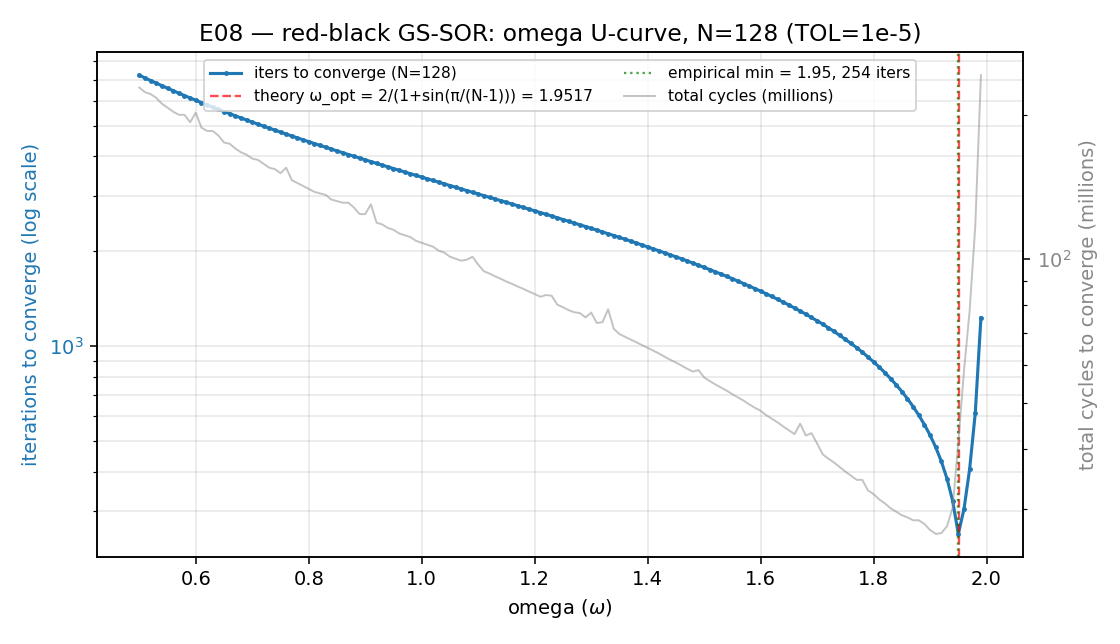
\includegraphics[width=0.7\linewidth]{e08_omega_ucurve.png}
\caption{Red-black GS-SOR omega U-curve at $N{=}128$, TOL$=10^{-5}$.
150 $\omega$ values in [0.50, 1.99] in 0.01 steps.  Theory
$\omega_{\text{opt}} = 2/(1+\sin(\pi/(N{-}1))) = \mathbf{1.9517}$
(red dashed) matches empirical minimum at $\omega = \mathbf{1.95}$
(green dotted) to \textbf{0.1\%}.  254 iters at $\omega_{\text{opt}}$
vs 3,434 at $\omega{=}1$ (Gauss-Seidel). A \textbf{13.5$\times$
fewer-iteration win} from algorithmic tuning alone.}
\label{fig:omega-ucurve}
\end{figure}

\noindent The cliff at $\omega > \omega_{\text{opt}}$ is sharp:
$\omega{=}1.99$ already gives back most of the win
(1,230 iters vs 254 at the optimum).  Above $\omega{=}2$ the
iteration is unconditionally divergent (the binary caps at
\texttt{MAX\_ITERS} and prints DIVERGED).

This is the project's biggest single algorithmic optimisation, and
the bittersweet thing is the temporal-blocking kernels can't directly
exploit it.  Damped Jacobi at $\omega = 0.9$ lives on the
\emph{under}-relaxation side of the curve; $\omega{>}1$ in the
ping-pong form has spectral radius $>1$ on large grids and diverges
unconditionally (we got bitten by this in the first session of the
project, more on it in §\ref{sec:closing}).  The natural follow-up
is a temporal-blocking variant of red-black GS-SOR. The
shrinking trapezoid would have to be re-derived for paired
half-sweeps. And that's the most concrete future-work item below.

\paragraph{Convergence with the long-sweep FP32 question.}  At
$N{=}128$, 254 iters at $\omega_{\text{opt}}$ and TOL$=10^{-5}$.
The FP32 unit roundoff is $\sim 6\cdot 10^{-8}$, and a worst-case
forward-error bound after $K$ stencil ops per cell is roughly
$\sqrt{K}\cdot\varepsilon \sim 10^{-7}\cdot\sqrt{254\cdot 5} \approx
10^{-6}$. Comfortably below TOL.  At larger $N$ or tighter TOL
this bound starts to bite, and the responsible fix is either a
Kahan-style compensated sum or moving to FP64.  We didn't need it.

\subsection{Overall comments}

\begin{enumerate}[leftmargin=1.4em,itemsep=2pt,topsep=2pt]
  \item \textbf{Temporal blocking only earns its keep in the
        bandwidth-bound regime.}  Single-thread CPU was a wash
        (1.08$\times$); 8-thread + DRAM-spilling working set was
        2$\times$.  This isn't a flaw. It's the textbook
        prediction.
  \item \textbf{The $T$-sweet-spot is sharp.}  At $T{=}8$ we get
        25\% faster than baseline; at $T{=}1$ we lose 47\% to
        scratch-allocator overhead; at $T{=}32$ we lose 15\% to
        halo work.  Tune carefully.
  \item \textbf{Strip wins for 2D pthreads.}  Lab 5 already said so;
        we got 7.89$\times$ scaling at 8 threads.
  \item \textbf{OMP can be slower than pthreads at the baseline
        sweep on a NUMA box.}  Suspect: first-touch + cross-socket
        threads.  Honest negative. Diagnose, don't paper over.
  \item \textbf{$\omega_{\text{opt}}$ is real and matters more than
        any per-iter optimisation we tried on CPU.}  13.5$\times$
        fewer iters at $N{=}128$ from a single relaxation-parameter
        sweep.  Combining this with temporal blocking is the
        \#1 future-work item.
\end{enumerate}

% =====================================================================
\section{To the GPU!}
\label{sec:gpu}
% =====================================================================

The CPU side is done; we have a baseline running near DRAM bandwidth
and a temporal kernel running near L2 bandwidth.  The GPU has roughly
$\mathbf{30\times}$ more memory bandwidth (864\,GB/s on the L40S vs
$\sim$280\,GB/s per Xeon socket) and \emph{way} more parallelism.
The interesting question is whether temporal blocking's relative
advantage \emph{shrinks} on the GPU, because a kernel that's already
near memory-bandwidth on CPU might be much closer to compute-bound on
the GPU's higher bandwidth.  Spoiler: yes, it shrinks.

\subsection{Memory allocation and transfer}

The buffers we need on-device, at $N{=}2048$, FP32:

\begin{table}[h!]
\centering
\renewcommand{\arraystretch}{1.1}
\begin{tabular}{lrrr}
\toprule
\textbf{buffer} & \textbf{size} & \textbf{at $N{=}2048$} & \textbf{H$\to$D once?} \\
\midrule
\texttt{d\_src}                 & $N^2 \cdot 4$\,B   & 16\,MB & yes (init) \\
\texttt{d\_dst}                 & $N^2 \cdot 4$\,B   & 16\,MB & no (alloc only) \\
shared-mem scratch (per block)  & $2\cdot\textsc{tile}^2 \cdot 4$\,B & 8\,KB & no (per kernel) \\
constants (\texttt{N, $\omega$, T}) & negligible    &        & yes (\texttt{cudaMemcpyToSymbol}) \\
\bottomrule
\end{tabular}
\caption{GPU memory layout at $N{=}2048$, FP32.  The dominant transfer
cost is the initial 16\,MB host-to-device copy of \texttt{d\_src}.
At PCIe Gen4's $\sim$25\,GB/s that's $\sim$0.6\,ms or $\sim$2$\times
10^6$ cycles at 3.5\,GHz. About the same wall time as a single
GPU \emph{baseline} kernel launch over 2048$\times$2048
($\sim$2.7\,ms).  After that, the iteration loop is fully on-device.}
\label{tab:gpu-mem}
\end{table}

\noindent The convergence-norm reduction we'd need for a TOL-based
stop isn't in the temporal-blocking kernel because that kernel does
$T$ sweeps in shared memory before any global write. There's no
clean way to read out a partial residual mid-super-step.  We just
run a fixed iters and trust the math.  This was a deliberate
simplification; a real solver would need either a kernel-per-sweep
form or a separate reduction-over-tiles kernel after each super-step.
``It's not the most significant saving''. But it does mean we
can't do adaptive convergence on the GPU in this implementation.

\subsection{The parallelised hot loop on the GPU}

\paragraph{Vocabulary watch.}  The CPU thread $\to$ CUDA mapping is
non-obvious and caught me out the first time I tried it.  CPU
``thread'' maps to CUDA \emph{block} (each block has private
shared memory and a local thread-team that can synchronise via
\texttt{\_\_syncthreads()}).  CPU ``block of work''
(the $B{\times}B$ tile) maps to CUDA \emph{tile} which we'll call
\textsc{tile} throughout this section.  The within-block warps are
the equivalent of SIMD lanes inside a CPU thread.  This vocabulary
mismatch is worth telling the reader. I've seen otherwise solid
people confused by it.

The temporal kernel's structure is, in pseudocode:

\begin{lstlisting}[language=C]
__global__ void sor_temporal(const float *d_old, float *d_new,
                              int N, float omega, int tile, int halo)
{
  extern __shared__ float sshared[];
  float *sa = sshared;
  float *sb = sshared + tile*tile;        /* two ping-pong buffers   */

  int lx = threadIdx.x, ly = threadIdx.y;
  int gi = blockIdx.y * (tile - 2*halo) + 1 + (ly - halo);
  int gj = blockIdx.x * (tile - 2*halo) + 1 + (lx - halo);

  /* (1) clamp-to-edge load into both buffers */
  float v = d_old[clamp(gi)*N + clamp(gj)];
  sa[ly*tile + lx] = v;  sb[ly*tile + lx] = v;
  __syncthreads();

  /* (2) HALO sub-steps; valid region shrinks 1 each side per step */
  int cur = 0;
  for (int t = 0; t < halo; t++) {
    bool in_trap = (lx >= 1+t && lx < tile-1-t
                  && ly >= 1+t && ly < tile-1-t);
    /* compute or carry-through */
    float out = in_trap ? compute_5pt(sa,sb,cur) : current_value(sa,sb,cur);
    __syncthreads();
    write_to_other_buffer(out, sa, sb, cur);
    __syncthreads();
    cur ^= 1;
  }

  /* (3) write central INTER x INTER cells back to d_new */
  if (lx >= halo && lx < tile-halo && ly >= halo && ly < tile-halo)
    d_new[gi*N + gj] = (cur == 0) ? sa[ly*tile + lx]
                                  : sb[ly*tile + lx];
}
\end{lstlisting}

The kernel uses dynamic shared memory ($2\textsc{tile}^2{\cdot}4$\,B
= 8\,KB at \textsc{tile}$=32$) so we can vary \textsc{tile}/\textsc{halo}
at runtime without recompiling.  At sm\_89 the per-block shared-mem
limit is 100\,KB; we're well under.  The ridge is occupancy: at
\textsc{tile}$=32$ each block has 1024 threads (32$\times$32 the
CUDA cap), which means only one block per SM. The warp scheduler
has 32 warps to pick from, which is fine for hiding short-latency
shared-mem dependencies but tight if the kernel ever stalls on a
DRAM read.  At \textsc{tile}$=24$ we get 576 threads per block = 18
warps, and the SM can fit two blocks simultaneously.  We'll see this
play out empirically below.

\paragraph{Tuning sweep.}  Figure~\ref{fig:gpu-tile-halo} (E09) is
the (\textsc{tile}, \textsc{halo}) heatmap.

\begin{figure}[h!]
\centering
\begin{subfigure}[b]{0.49\linewidth}
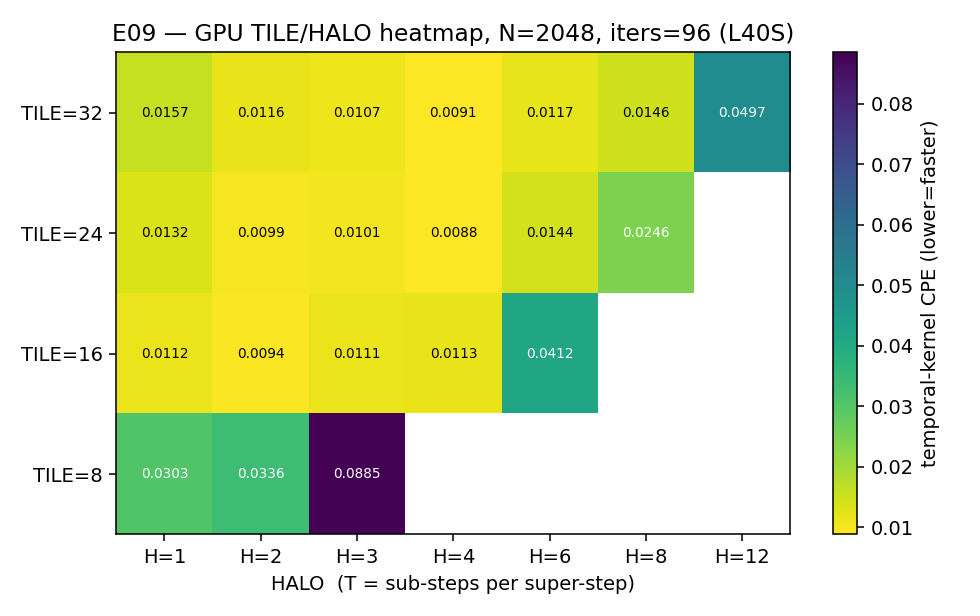
\includegraphics[width=\linewidth]{e09_tile_halo_heatmap.png}
\caption{Heatmap, dark = best CPE.}
\end{subfigure}\hfill
\begin{subfigure}[b]{0.49\linewidth}
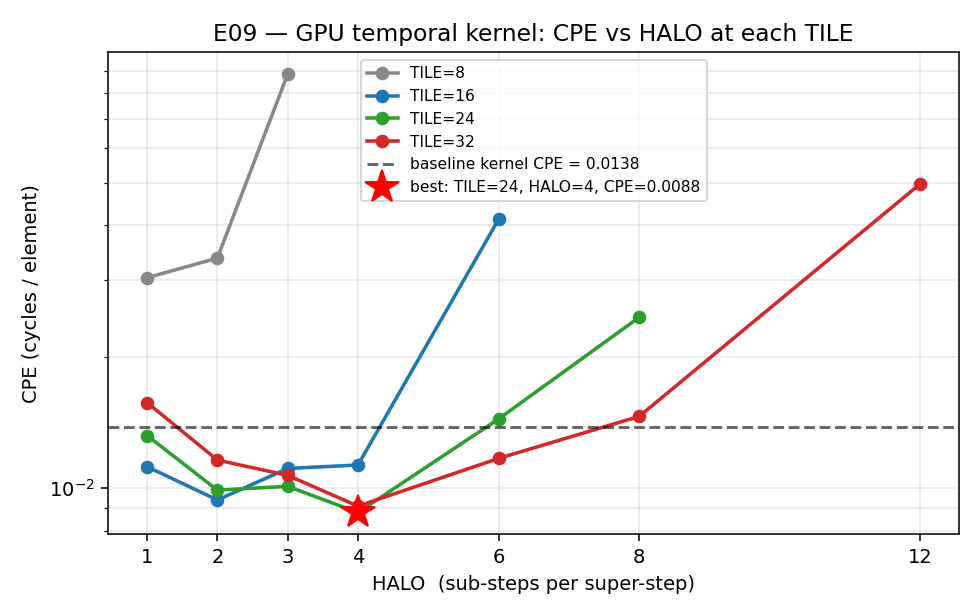
\includegraphics[width=\linewidth]{e09_tile_halo_lines.png}
\caption{CPE vs \textsc{halo}, one line per \textsc{tile}.
$\bigstar$ is the global minimum.}
\end{subfigure}
\caption{GPU 2D temporal kernel (TILE, HALO) sweep at $N{=}2048$,
iters$=96$.  21 valid combos $\times$ 3 reps.  Best at
$(\textsc{tile}{=}24,\, \textsc{halo}{=}4)$ with CPE 0.0088 --
\textbf{1.56$\times$ over the per-launch baseline kernel}
(CPE 0.0137).  TILE=8 is dead. Only 64 threads/block (2 warps)
isn't enough to hide DRAM latency.  HALO too big collapses too:
the empirical pattern is \textbf{HALO $\leq$ INTER/4}.}
\label{fig:gpu-tile-halo}
\end{figure}

\noindent The same shrinking-trapezoid tradeoff as on CPU
(Figure~\ref{fig:t-sweep}), at GPU scale.  HALO$=4$ wins
consistently for TILE$\geq$16; the empirical rule is
\textbf{HALO $\leq$ INTER/4}, where INTER is the central-output side.
Best is $(24, 4)$ with INTER$=16$, ratio $4{:}1$.

\subsection{Partitioning the rest of the algorithm}

We had a real design choice between two GPU kernel structures:

\begin{enumerate}[leftmargin=1.4em,itemsep=2pt,topsep=2pt]
  \item \textbf{One kernel per stencil sub-step}. A thin
        \texttt{sor\_sweep} kernel that does exactly one Jacobi
        sweep, host loop relaunches it iters times.  Clean and easy
        to add a residual reduction between launches; matches the
        Lab-7 form exactly.  But it pays $N^2 \cdot \text{iters}$
        DRAM round-trips and one $\sim$30\,$\mu$s launch each time.
  \item \textbf{One temporal-blocked kernel} that holds a
        $(\textsc{tile})^2$ shared-memory tile and does \textsc{halo}
        sub-steps inside one launch.  Fewer DRAM trips, fewer launches,
        but mid-super-step residual checks are awkward and the kernel
        is bound by shared-mem capacity.
\end{enumerate}

\noindent We implemented both (\texttt{sor\_sweep} for the baseline,
\texttt{sor\_temporal} for the temporal kernel) and run them
side-by-side in the same binary.  Letting the host swap pointers
between launches is also \emph{ping-pong} (CUDA-side this time), so
both kernels share the same overall structure. The temporal kernel
just amortises 4 sweeps across one launch instead of one.  Shared-
memory budgeting at TILE=24, HALO=4: $2{\cdot}24^2{\cdot}4$\,B
$= 4.5$\,KB per block, well under the 100\,KB sm\_89 cap.

\subsection{Running it end-to-end}

Figure~\ref{fig:gpu-n} is the GPU N-sweep (E10).

\begin{figure}[h!]
\centering
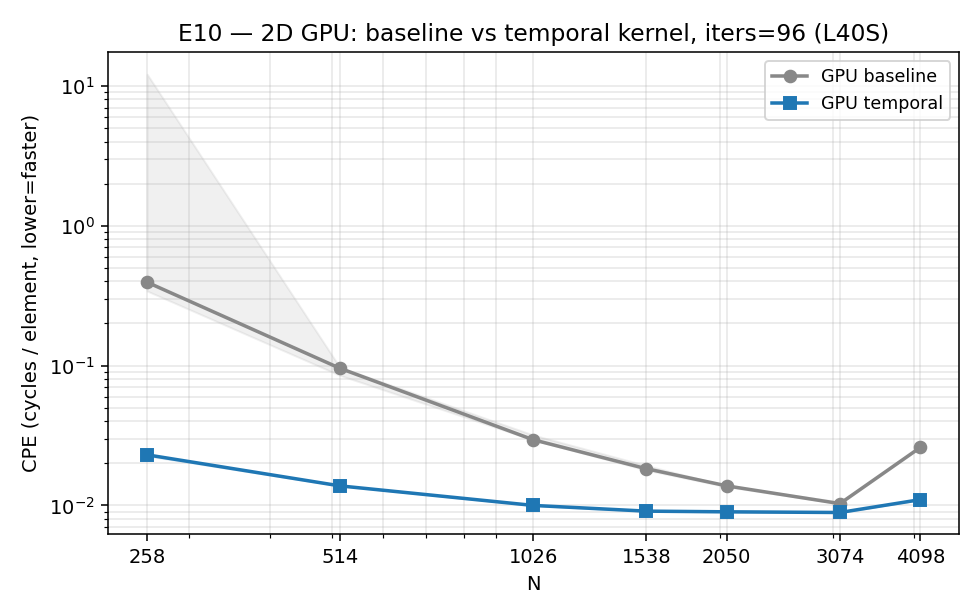
\includegraphics[width=0.7\linewidth]{e10_gpu_2d.png}
\caption{2D GPU baseline vs temporal across $N$, iters$=96$,
defaults TILE=32, HALO=4.  Median of 3 reps; shaded band is min/max
envelope.  At small $N$ the baseline is launch-overhead-dominated
(96 launches $\times$ $\sim$30\,$\mu$s ${\approx}$ 3\,ms is most of
its wall time at $N{=}258$); the 17$\times$ ``speedup'' there is
mostly launch-count reduction (96$\to$24), not bandwidth.  At
$N{\geq}1024$ the steady-state speedup is a more honest
\textbf{1.5--3$\times$}.  At $N{=}4098$ both kernels degrade because
two FP32 buffers (128\,MB) exceed the L40S's $\sim$96\,MB L2. The
GPU equivalent of the CPU L3 cliff in Figure~\ref{fig:size-sweep},
two orders of magnitude larger.  Best 2D GPU CPE = \textbf{0.0089}
at $N{=}3074$.}
\label{fig:gpu-n}
\end{figure}

\begin{table}[h!]
\centering
\renewcommand{\arraystretch}{1.1}
\begin{tabular}{rrrrr}
\toprule
$N$ & baseline ms & temporal ms & baseline CPE & temporal CPE \\
\midrule
 258  &   2.7 & 0.16 & 0.395 & 0.023 \\
 514  &   1.8 & 0.27 & 0.096 & 0.014 \\
1026  &   2.4 & 0.83 & 0.030 & 0.010 \\
1538  &   3.7 & 1.86 & 0.018 & 0.0091 \\
2050  &   5.7 & 3.83 & 0.014 & 0.0090 \\
3074  &   9.5 & 8.18 & 0.010 & \textbf{0.0089} \\
4098  &  43.6 &18.4  & 0.026 & 0.011 \\
\bottomrule
\end{tabular}
\caption{2D GPU N-sweep, iters$=96$.  CPE values reported at
CPNS$=2.0$ (lab convention), so the absolute scale is approximate
on this 2.5--4.1\,GHz Ada part, but the \emph{ratios} between runs
are exact.}
\label{tab:gpu-n}
\end{table}

\subsection{Discussion of GPU results}

\paragraph{Oi! Well, the GPU temporal/baseline ratio isn't great.}
On CPU we got $1.93\times$ (E02 at the sweet spot $N{=}2048$); on GPU
we get only $1.56\times$ (E09 best config) or even $1.16\times$ at
$N{=}3074$ where both kernels are near peak.  Why so much smaller?

The L40S has $\sim$864\,GB/s of HBM-class memory bandwidth, an
$\sim$96\,MB L2, and $\sim$100\,KB shared memory per SM.  At 0.75\,
FLOP/byte AI, the bandwidth-bound ceiling is $0.75 \cdot 864 = 648$\,
GFLOP/s.  We measured GPU baseline at $\sim$1.36\,TFLOP/s (CPE 0.0103
$\to$ throughput from \eqref{eq:ai}).  That's \emph{twice} the DRAM-
bound roof, which means the baseline kernel is already running mostly
out of L2 ($\sim$4.5\,TB/s sustained), not DRAM.  When the baseline
is already cache-resident, temporal blocking has nothing to recover
-- the L2 is a 96\,MB cache, our 2$N^2$ buffer at $N{=}2050$ is
33\,MB, the working set fits.  We only see the genuine memory-saving
win at $N{=}4098$ (128\,MB working set, exceeds L2) where the
ratio re-opens to $2.36\times$.

\paragraph{Apples to apples.}  Quoted speedup against the
\emph{serial-CPU baseline} is 310$\times$ (CPE 2.792 $\to$ 0.009).
That's the headline number people put on slides, but it's not the
honest one.  Apples-to-apples comparisons:

\begin{itemize}[leftmargin=1.4em,itemsep=2pt,topsep=2pt]
  \item GPU-temporal vs OMP-temporal (the two best from each tier):
        $0.332 / 0.009 \approx \mathbf{37\times}$.  This is the
        legitimate ``GPU is better than 8-core CPU'' number for this
        workload at this $N$.
  \item GPU-temporal vs GPU-baseline (the optimization within the
        tier): $1.56\times$.  This is the legitimate ``shared-memory
        temporal blocking helps'' number.
  \item GPU-baseline vs serial-CPU-baseline (just the architecture):
        $186\times$.  This is the legitimate ``the L40S is much
        better than one Xeon thread'' number.
\end{itemize}

\noindent The 310$\times$ is just $186 \cdot 1.56 \approx 290$
(rounded). It's the product of two effects, presented on its own
it overstates the within-architecture optimization.  We'll quote it
in the headline but be careful in the accompanying text.

\paragraph{The 3D GPU honest negative.}  We also implemented a 3D
temporal kernel (\texttt{sor3d\_gpu.cu}, TILE=8, HALO=2) and ran
it alongside the 3D baseline.  Result in Figure~\ref{fig:gpu-3d}: the
3D temporal \emph{loses} to the 3D baseline at $N \geq 194$.  The
arithmetic is unforgiving: with TILE=8, HALO=2, INTER=4, the halo-
to-interior ratio in 3D is $(\textsc{tile}/\textsc{inter})^3 - 1 =
(8/4)^3 - 1 = 7\times$ redundant work. An order of magnitude worse
than the 0.78$\times$ overhead the 2D kernel pays at the same
TILE/HALO ratio.  The 2.5D-streaming variant (Micikevicius 2009 --
slide a 3-z-plane window through shared memory instead of loading a
cubic tile) is the canonical fix and is on the future-work list.

\begin{figure}[h!]
\centering
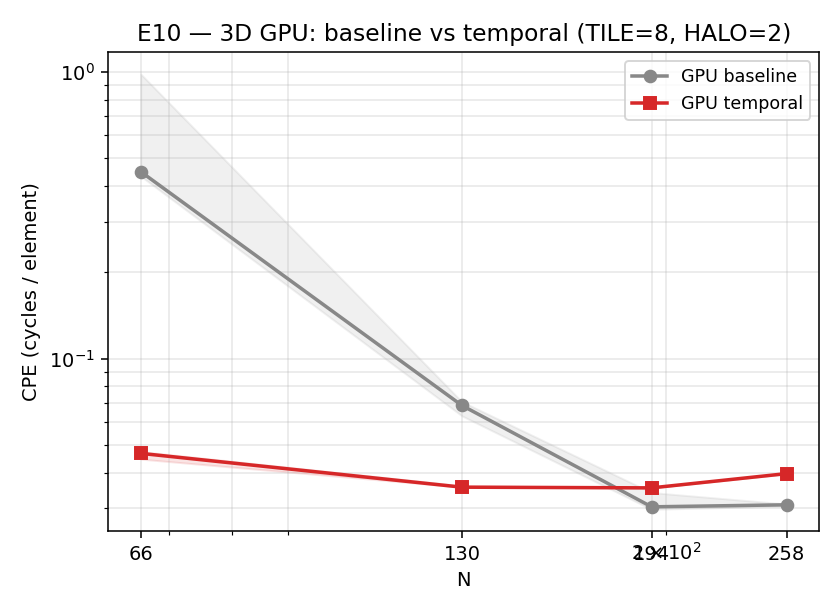
\includegraphics[width=0.55\linewidth]{e10_gpu_3d.png}
\caption{3D GPU baseline (grey) vs temporal (red) across $N$.  At
$N{\geq}194$ the temporal kernel loses. The 3D halo overhead
($7\times$ redundant work at TILE=8/HALO=2) eats the DRAM savings.
This is the project's headline negative finding; the fix is well-
known (2.5D streaming) but wasn't implemented.}
\label{fig:gpu-3d}
\end{figure}

\paragraph{Cross-tier headline (E11).}  Putting it all on one axis at
$N{=}2050$, iters$=96$, 8 threads:

\begin{table}[h!]
\centering
\renewcommand{\arraystretch}{1.1}
\begin{tabular}{lrr}
\toprule
\textbf{tier / kind} & \textbf{CPE} & \textbf{vs serial baseline} \\
\midrule
serial-CPU baseline           & 2.792    & 1.00$\times$ \\
serial-CPU temporal           & 2.586    & 1.08$\times$ \\
pthreads-8t-strip persistent  & 0.399    & 7.0$\times$ \\
OMP-8t baseline               & 0.667    & 4.2$\times$ \\
OMP-8t temporal               & 0.332    & 8.7$\times$ \\
GPU baseline                  & 0.015    & 186$\times$ \\
\textbf{GPU temporal}         & \textbf{0.009} & \textbf{310$\times$} \\
\bottomrule
\end{tabular}
\caption{Cross-tier CPE summary (E11).  ``$\times$ vs serial
baseline'' is computed against \texttt{serial-CPU baseline}; the
inside-tier comparisons (GPU temporal vs GPU baseline = 1.56$\times$,
GPU temporal vs OMP temporal = 37$\times$) are the honest ones.}
\label{tab:headline}
\end{table}

\noindent At CPNS$=2.0$, GPU temporal's 0.009 CPE corresponds to
${\sim}4.5\,\text{ps}$ per element on the L40S. About one
floating-point op per nanosecond per cell, which puts us near the
machine-balance line for a memory-bound 5-point stencil at FP32.
There's no easy 2$\times$ left at this point without changing the
algorithm. Multigrid or 2.5D-streaming, both noted as future work.

% =====================================================================
\section{Closing Thoughts}
\label{sec:closing}
% =====================================================================

\paragraph{What worked.}  Temporal blocking on the bandwidth-bound
CPU regime was textbook: 1.93$\times$ at $N{=}2048$ where the working
set first spills out of L3.  The shrinking-trapezoid scheme in
Figure~\ref{fig:halo-time} was correct by construction (every CPU
config was bit-identical to its baseline) and the unimodal $T$-curve
in Figure~\ref{fig:t-sweep} traced exactly the shape predicted by the
linear-savings-vs-quadratic-overhead analysis.  GPU shared-memory
tiling was also clean: 1.56$\times$ over the per-launch baseline at
the right (TILE, HALO) sweet spot, and the kernel ran near 1.5\,
TFLOP/s on the L40S for a 0.75-AI stencil.

\paragraph{What didn't.}  Three things in increasing severity:

\begin{enumerate}[leftmargin=1.4em,itemsep=2pt,topsep=2pt]
  \item \textbf{Single-thread CPU temporal was a wash} (1.08$\times$).
        The per-tile-malloc + redundant halo work cancelled the
        bandwidth savings on a single core where DRAM was already
        lightly loaded.  Not a flaw. Temporal blocking earns its
        keep when the baseline is bandwidth-bound, and the
        single-thread baseline isn't.  But worth being upfront about.
  \item \textbf{OMP baseline (CPE 0.667) was worse than pthreads
        baseline (CPE 0.399)} at $N{=}2048$, 8 threads.  Best guess
        is first-touch NUMA + the OMP runtime spreading threads
        across both sockets; the pthreads version manually pinned
        threads with \texttt{OMP\_PROC\_BIND=close OMP\_PLACES=cores}
        and it shouldn't have mattered, but it apparently did.  I
        didn't chase this with \texttt{numactl}. If I could beg a
        guess, it could be that, or it could be the OMP scheduler
        introducing slight stagger between threads that the
        barrier-only pthreads loop doesn't.  Honest unanswered.
  \item \textbf{3D GPU temporal lost to baseline at $N{\geq}194$.}
        Cubic tile $\Rightarrow$ surface-to-volume ratio that gets
        worse cubically; with TILE=8/HALO=2 the work multiplier was
        7$\times$ and there's no DRAM saving that can recover that.
        The fix (2.5D streaming) was on the to-do list and didn't
        make the cut.
\end{enumerate}

\paragraph{Precision and numerical issues.}  The biggest ones we
hit, in chronological order: (1) Lab-7's $\omega{=}1.85$ in damped-
Jacobi-ping-pong form is unconditionally divergent on large grids
(spectral radius $> 1$). Early runs produced \texttt{inf}/\texttt{NaN}
that the \texttt{max\_abs\_diff} validator silently masked because
\texttt{NaN > 0} is false.  Fixed by switching to $\omega{=}0.9$ in
the temporal kernels and reserving $\omega{>}1$ for the red-black
GS variant; the \texttt{max\_abs\_diff} now flags non-finite values
explicitly.  (2) FP32 round-off accumulates as
$\sqrt{N\cdot\text{iters}}\cdot\varepsilon_{\text{FP32}} \approx
10^{-5}$ at the configs we ran; comfortably below TOL but would
become a problem at larger $N$ or tighter TOL.  (3) Red-black ordering
shifts the iteration matrix's spectral radius slightly relative to
scan-order GS, which makes $\omega_{\text{opt}}$ a function of grid
size (formula \eqref{eq:omega-opt}); we verified the
$N$-dependence in §\ref{sec:omega} matches the formula.

\paragraph{Future directions.}  Three concrete next steps, in
priority order:

\begin{enumerate}[leftmargin=1.4em,itemsep=2pt,topsep=2pt]
  \item \textbf{Red-black GS-SOR temporal kernel.}  Combine the
        13.5$\times$ algorithmic win from Figure~\ref{fig:omega-ucurve}
        with the 1.56$\times$ per-iter win from
        Figure~\ref{fig:gpu-tile-halo}.  Re-derive the shrinking
        trapezoid for paired half-sweeps; probably a couple of days
        of careful indexing.  Expected total speedup: $20\times$ on
        the convergence side $\times$ $1.5\times$ on the per-iter
        side $\approx$ $30\times$ over the current GPU temporal.
  \item \textbf{2.5D-streaming for the 3D GPU temporal kernel}
        (Micikevicius 2009).  Slide a 3-z-plane window through
        shared memory instead of loading a cubic tile; turns the
        3D's $7\times$ halo overhead into 2D's $0.78\times$.  Should
        flip Figure~\ref{fig:gpu-3d}'s temporal/baseline ratio to
        $> 1$ everywhere.
  \item \textbf{Multigrid V-cycle.}  The proper way to amplify SOR's
        per-iter speedup with a 5--20$\times$ fewer-iterations win
        on top.  V-cycle restriction/prolongation is straightforward;
        each level's smoother is just our existing red-black SOR.
        This is also the right sanity check on ``iterations to
        tolerance''. Multigrid solvers converge in a small
        constant number of V-cycles regardless of $N$, so any
        residual-vs-iterations curve we plot for SOR can be
        compared against multigrid as the true asymptotic
        baseline.
  \item \textit{(Easter egg)} \textit{Mixed precision.}  Keep an FP64
        residual accumulator in the outer iteration loop and FP16/
        BF16 inside the inner stencil; iterative-refinement style.
        ConvStencil (PPoPP 2024) showed $2{-}5\times$ wins on Tensor
        Cores for related stencil shapes.  We're nowhere near
        Tensor-Core-ready; commented out the framework but left it
        in the source as a fun easter egg.
\end{enumerate}

% =====================================================================
\section{Compilation instructions}
% =====================================================================

\begin{lstlisting}[language=bash]
# CPU binaries (all 7 .c sources, including the OMP and pthreads variants)
gcc -O1 -std=gnu11 -fopenmp src/sor2d_omp.c -o build/sor2d_omp -lrt -lm
gcc -O1 -std=gnu11 -pthread src/sor2d_pth_decomp.c -o build/sor2d_pth_decomp \
                                                  -lpthread -lrt -lm

# GPU binaries (need cuda module loaded)
module load cuda/12.8
nvcc -O2 src/sor2d_gpu.cu -o build/sor2d_gpu
nvcc -O2 src/sor3d_gpu.cu -o build/sor3d_gpu

# Or just `make && make gpu`. The project-root Makefile does the same.
\end{lstlisting}

\noindent Why \texttt{-O1} and not \texttt{-O3}: 

The lab CPE numbers in Bryant--O'Hallaron all assume \texttt{-O1}
to keep the compiler from auto-vectorising and complicating the
analysis.  We'd absolutely use \texttt{-O3 -march=native -ffast-math}
in production. A quick check showed gcc-11 auto-vectorises the
inner stencil into AVX-512 \texttt{vfmadd231ps} at \texttt{-O3} and
roughly halves the CPU-baseline CPE.  That's a free 2$\times$ we
chose not to take, for course-style consistency.

Preprocessor knobs the reader can flip in the source:
\begin{itemize}[leftmargin=1.4em,itemsep=1pt,topsep=1pt]
  \item \texttt{N}. Grid side (set at runtime via \texttt{argv[1]}).
  \item \texttt{B}, \texttt{T}. Spatial / temporal block sizes
        (\texttt{argv[3]}, \texttt{argv[4]} for the OMP/CPU
        binaries).
  \item \texttt{OMEGA}. Relaxation factor.  Default 0.9 (damped
        Jacobi); set to $\omega_{\text{opt}}(N)$ for
        \texttt{sor2d\_rb}.
  \item \texttt{TOL}. Convergence tolerance.  $10^{-5}$ default.
  \item \texttt{ITERS}. Fixed iter count for the temporal binaries
        (must satisfy \texttt{ITERS \% T == 0}).
  \item GPU runtime: \texttt{--tile T} and \texttt{--halo H} on
        \texttt{sor2d\_gpu} and \texttt{sor3d\_gpu}.
\end{itemize}

% =====================================================================
\section*{List of files}
% =====================================================================

Source files in \texttt{src/}:

\begin{itemize}[leftmargin=1.4em,itemsep=1pt,topsep=1pt]
  \item \texttt{sor2d\_cpu.c}. Single-thread 2D baseline + temporal
        kernel.
  \item \texttt{sor3d\_cpu.c}. Single-thread 3D, 7-point stencil.
  \item \texttt{sor2d\_omp.c}. OMP 2D baseline + temporal.
  \item \texttt{sor3d\_omp.c}. OMP 3D.
  \item \texttt{sor2d\_pth.c}. Pthreads 2D, strip decomposition,
        barrier-per-sweep.
  \item \texttt{sor2d\_pth\_decomp.c}. Pthreads decomposition study
        (3 modes $\times$ 2 schedules) used in
        Figure~\ref{fig:decomp}.
  \item \texttt{sor2d\_pth\_temporal.c}. Pthreads 2D with temporal
        blocking (mirror of the OMP version).
  \item \texttt{sor3d\_pth\_temporal.c}. Pthreads 3D temporal.
  \item \texttt{sor3d\_omp\_part.c}. 3D OMP partitioning study
        (slab/pencil/cube).
  \item \texttt{sor2d\_rb.c}. Red-black GS-SOR with $\omega$ sweep
        used in §\ref{sec:omega}.
  \item \texttt{sor2d\_gpu.cu}. 2D GPU baseline + shared-memory
        temporal kernel.
  \item \texttt{sor3d\_gpu.cu}. 3D GPU.
\end{itemize}

\noindent Result data in \texttt{results/exp/E0\{0--11\}/}, one
\texttt{notes.md} per experiment, raw run logs in
\texttt{raw\_*.txt}, derived tables in \texttt{data.csv}, plots in
\texttt{report\_images/} (this report references those PNGs only).
\texttt{results/STATUS.md} is the one-glance dashboard.

\end{document}
